%%%%%%%%%%%%%%%%%%%%%%%%%%%%%%%%%%%%%%
\documentclass[a4paper,english]{report}    % list options between brackets

\RequirePackage{color}
\RequirePackage{float}
\RequirePackage{amsfonts}
\RequirePackage{amsmath}
\RequirePackage{alltt}
\RequirePackage{ae}
\RequirePackage{times}
\RequirePackage{fancyhdr}
\RequirePackage{graphicx} 
\RequirePackage{makeidx}  
\RequirePackage{wrapfig}

\RequirePackage{hyperref}

\UseRawInputEncoding

\hypersetup{
    bookmarks=true,         % show bookmarks bar?
    unicode=false,          % non-Latin characters in Acrobat�s bookmarks
    pdftoolbar=true,        % show Acrobat�s toolbar?
    pdfmenubar=true,        % show Acrobat�s menu?
    pdffitwindow=false,     % window fit to page when opened
    pdfstartview={Fit},    % fits the width of the page to the window
    pdftitle={Elmer GUI Tutorials},    % title
    pdfauthor={CSC - IT Center for Science},     % author
    pageanchor=true,
    hyperindex=true,
    pdfnewwindow=true,      % links in new window
    colorlinks=true,       % false: boxed links; true: colored links
    linkcolor=black,          % color of internal links
    citecolor=black,        % color of links to bibliography
    filecolor=black,      % color of file links
    urlcolor=black           % color of external links
}
 
\makeindex             
  

% Use these to make the printable area bigger
% Also have the option 'ownsize' active in the documentclass
\setlength{\hoffset}{-15mm}
\setlength{\voffset}{-10mm}
\addtolength{\textwidth}{30mm}
\addtolength{\textheight}{20mm}
%\addtolength{\headwidth}{30mm}


% Command file syntax stuff
\definecolor{SifCol}{rgb}{0.5,0.5,0.5}
%\definecolor{SifCol}{rgb}{1,1,1}

% Index for keywords
\newcommand{\sifitem}[2]{\item[\tt{#1}]\index{#1}\hspace{1mm}{\color{SifCol}\hspace{1mm}\tt{#2}}\newline} 
%item with two fields but no text
\newcommand{\sifitemnt}[2]{\item[\tt{#1}]\index{#1}\hspace{1mm}{\color{SifCol}\hspace{1mm}\tt{#2}}} 


\newcommand{\sifbegin}{\begin{description}}
\newcommand{\sifend}{\end{description}}
\newcommand{\modinfo}[2]{{\bf{#1}}: {#2}\newline}

\newcommand{\ttbegin}{\begin{alltt}}
\newcommand{\ttend}{\end{alltt}}
\newcommand{\ttitem}[1]{\item[\tt{#1}]\mbox{}\\}
\newcommand{\keno}{$\backslash$}


\newcommand{\Sf}[1]{\textsf{#1}}
\newcommand{\Bf}[1]{{\sffamily\bfseries}}

\newcommand{\URL}[1]{\texttt{#1}}

% Some new commands...
\def\xwin{X Window System}
\def\xbr{Xbrowse}
\def\prag{\Tt{\#pragma}}

\newcommand{\inxgra}[2]{{\centerline{\includegraphics[width=#1]{#2}}}}
\newcommand{\inygra}[2]{{\centerline{\includegraphics[height=#1]{#2}}}}
\newcommand{\incgra}[2]{{\centerline{\includegraphics[height=#1]{#2}}}}

\providecommand{\ftn}{Fort\-ran~90}
\providecommand{\Idx}[1]{{#1}\index{#1}}


%%%%%%%%%%%%%%%% Math definitions for Elmer Solver Manuals %%%%%%%%%%%%%%%%%
\newcommand{\Bfm}[1]{\mbox{\boldmath{${#1}$}}}

\newcommand{\tensorspace}[1]{\boldsymbol{#1}}         % Sets of tensors are bold italic
\newcommand{\tensor}[1]{\boldsymbol{#1}}              % Tensors are bold italic
\newcommand{\point}[1]{\mathbf{#1}}                   % Points are bold upright
\newcommand{\pointf}[1]{\mathbf{#1}}                  % Point-valued functions are bold upright
\newcommand{\pointfm}[1]{\mbox{\boldmath{${#1}$}}}    % Point-valued functions for math symbols

\DeclareMathOperator{\grad}{\mathbf{grad}}            % The spatial gradient operator
\newcommand{\Grad}{\mbox{\boldmath{${\nabla}$}}}      % gradient with respect to the points of the reference configuration
\DeclareMathOperator{\curl}{\mathbf{curl}}            % The spatial curl operator
\DeclareMathOperator{\Curl}{\mathbf{Curl}}            % curl with respect to the points of the reference configuration
\DeclareMathOperator{\rot}{\mathbf{rot}}              % rot operator defined for scalars
\DeclareMathOperator{\divs}{\mathrm{div}}             % scalar-valued divergence
\DeclareMathOperator{\divvec}{\mathbf{div}}           % vector-valued divergence
\DeclareMathOperator{\Divvec}{\mathbf{Div}}           % vector-valued divergence w. r. t. the points of the reference configuration
\newcommand{\Div}{\nabla\cdot}                        

%\newcommand{\Vec}[1]{\vec{#1}}
%\newcommand{\Vec}[1]{\mathify{\mathbf{#1}}}

%\newcommand{\Matr}[1]{\mbox{${#1}$}}                  % Matrices are just italic to differentiate between true tensors and matrices
\newcommand{\Matr}[1]{{#1}}                     % Matrices
\newcommand{\Der}[2]{\frac{\partial{#1}}{\partial{#2}}}
\newcommand{\Secder}[2]{\frac{\partial^2{#1}}{\partial{#2}^2}}
\newcommand{\Inv}[1] {\frac{1}{#1}}


% Make the headings fancier
\pagestyle{fancy}

\lhead[\normalfont\small\bf\thepage]{\normalfont\small\slshape\rightmark}
\rhead[\small\slshape\lefthead]{\normalfont\small\bf \thepage}
%\setlength{\headrulewidth}{0.4pt}
%\renewcommand{\chaptermark}[1]{\markright{\bf \chaptername \ \thechapter.\ #1}{}}
%\renewcommand{\chaptermark}[1]{\markright{\bf \thechapter.\ #1}{}}
\renewcommand{\sectionmark}[1]{}
\renewcommand{\subsectionmark}[1]{}
\cfoot{}

% This sets the Elmer version in the documentation
%\newcommand{\elmerversion}{6.0}



% This sets the Elmer version in the documentation
\newcommand{\elmerversion}{8.4}


\title{\Huge{\bf Get Started with LaTeX\\ for use with Elmer Tutorials}}
\author{Rich Bayless }

\begin{document}
\maketitle

\chapter*{Get Started with Elmer}

\section*{About this document}

This document, Get Started with Elmer, is intended to help anyone who has just downloaded Elmer and would like some help getting started.\\

The first three chapters are provided specifically for Windows users, with detailed instructions to download, install, and start using Elmer.  The instructions have been tested on Windows 10.\\

The rest of the chapters in this document generally apply to all users, running Windows, Linux, and MacOS.\\

Topics discussed include:

\begin{itemize}
  \item Paraview and ElmerVTK for post processing Elmer results
  \item Using Elmer, where to find test cases, tutorials, the Elmer user forum, and youtube video
  \item Parallel operation of Elmer
  \item External tools with Elmer, such as Gmsh and Salome, providing examples of creating multiple bodies
  \item Elmerfem Wiki, a copy of the old wiki
  \item Installing the Elmer Virtual Machine
  \item Installing Elmer in Linux
\end{itemize}


The present manual corresponds to Elmer software version~\elmerversion{}.\\

Latest documentations and program versions of Elmer are available (or links are provided) at \url{http://www.csc.fi/elmer}. \\

\section*{Copyright information}

This document is licensed under the Creative Commons Attribution-NonCommerical 3.0 License.  To view a copy of this license, visit \url{http://creativecommons.org/licenses/by-nc/3.0/}.\\

Initially this document, Get Started with Elmer, has been written by Rich Bayless.  External contributions are welcome.





\pagestyle{empty}

% Table of contents:
\setcounter{secnumdepth}{2}%
\setcounter{tocdepth}{2}  % set this to 1 in the final version

\phantomsection
\addcontentsline{toc}{part}{Table of Contents}
\tableofcontents


\newpage

\renewcommand{\chaptername}{Chapter}

% change the plain style used for chapter pages
\fancypagestyle{plain}{
\lhead{}
\rhead{}
\rfoot{
\includegraphics[width=18mm]{by-nc}}
\lfoot{\footnotesize{CSC -- IT Center for Science}}
\chead{}
%\cfoot{\bfseries \thepage}
\cfoot{}
\renewcommand{\headrulewidth}{0.0pt}
}

% and the fancy style used elsewhere
\pagestyle{fancy}
\rhead{\bfseries \thepage}
\lhead{\bfseries \rightmark}
\rfoot{
\includegraphics[width=18mm]{by-nc}}
\lfoot{\footnotesize{CSC -- IT Center for Science}}
\chead{}
\cfoot{}
\renewcommand{\headrulewidth}{0.4pt}
\renewcommand{\footrulewidth}{0.4pt}
%

\clearpage

\graphicspath{{./}{TexStart/}}
\chapter{Get Started with LaTeX}

\modinfo{Directory}{TexStart}
\modinfo{Author}{Rich Bayless}


\section{Purpose}

The Elmer tutorials are written using LaTeX, which is a powerful tool.  Like any favourite tool, once you know a little about how to use that tool, it will become second nature for its use.  To help turn a steep learning curve into a gentle on-ramp, the following examples that use TexWorks will help one get started with editing of Elmer tutorials, or to create new Elmer tutorials.  These instructions should work with just about any LaTeX editor, since these are the basics of working with LaTeX documents.\\

Adding graphics to Elmer tutorials provide a great visual aid for subjects that can otherwise be dry and hard to comprehend. Examples of various graphics formats are provided, with the intention that they can be copied and pasted into another .tex file.  Instead of reinventing the wheel, let's keep a record of what works for the Elmer tutorials.\\

If any of you out there have spent an hour or two trying to figure out how to add the perfect graphic, in the perfect format, and in just the right location using Texworks or other LaTeX editors, then this may be the right spot for you to pass on your knowledge.


\section{Examples}

Note that the full explanation for each example is given in the .tex file. There may be an explanation in the text of the .pdf, but look at the .tex source for the real story.\\

We'll  start with the basics of controlling lines and paragraphs and work our way up into more complicated examples.\\


For graphics, we will use a blank yellow picture, with a 20 pixel wide black border.  Various sizes of pictures, such as 1000 pixels wide by 200 pixels high, are used.  When picking an example, consider the approximate size of your desired figure and the aspect ratio.  The size of your desired figure does not need to match any of these examples. The graphics are just guidelines, nothing more than that.\\

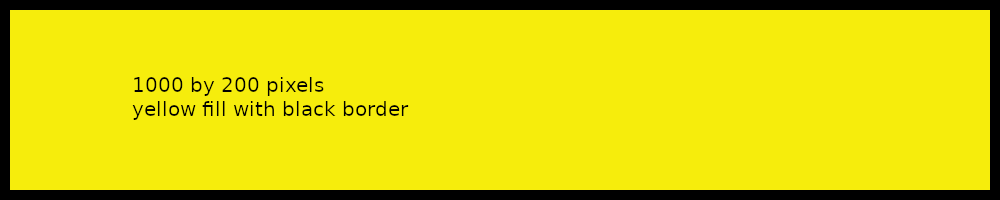
\includegraphics{1000x200}

% end that section and start again on a new page
\newpage

\chapter{Lines and paragraphs}

\section{Lines and paragraphs, what to do}

Here are several text examples that show how to control lines and paragraphs.   TexWorks and LaTeX work a little differently than the typical text editor that you may have used, specifically one needs to use a double return to end a paragraph.\\

If you want to start a new indented paragraph, just add a double return. Nam dui ligula, fringilla a, euismod sodales, sollicitudin vel, wisi.  Morbi auctor lorem non justo. Nam lacus libero, pretium at, lobortis vitae, ultricies et, tellus.

If you want a blank line after the first paragraph and to start a second indented paragraph, add a double backslash and a double return, in that order.  Donec aliquet, tortor sed accumsan bibendum, erat ligula aliquet magna, vitae ornare odio metus a mi.  Cras nec ante. Pellentesque a nulla.\\

Here is the beginning of the requested second paragraph. Cum sociis natoque penatibus et magnis dis parturient montes, nascetur ridiculus mus. Aliquam tincidunt urna. Nulla ullamcorper vestibulum turpis. Pellentesque cursus luctus mauris.\\

Use double returns to end a paragraph, or use double backslashes and double returns to end a paragraph.

\section{Lines and paragraphs, what NOT to do}

In terms of style, IMHO, the use of single returns should be discouraged.  Single returns will create a simulated word wrap, that doesn't show up in the published .pdf document.
This line starts with a single return and ends with a single return.
The next line shows up in the .pdf document as if the single return didn't exist.  In your TeXworks editing windows, the single return shows up as a break in word wrapping.  To see what this means, adjust the width of the TeXworks editing window from full width, to half width, to quarter width.  The other paragraphs without the single return all work wrap nicely, while this paragraph with the single return will not word wrap nicely.  It's a habit learned with other text editors, to end each line with a return, so it will be hard to change just while using TeXworks, but once you get used to letting TeXworks take care of word wrapping for you, using TeXworks will get easier.\\

Likewise, in terms of style, IMHO, the use of double backslashes in the middle of a paragraph should be discouraged. Curabitur dictum gravida mauris.  Here comes a double backslash without a return.\\ Note that the next line is not indented.  Pretty ugly, there may be a time when you will need to use an early line ending, but typically please don't do it.\\

Note:  Please follow these guidelines while creating new documents, and possibly while editing old documents.  Particularly, when the documents are under source control, such as git, editing existing documents solely to change what is strictly formatting, is frowned upon.  In other words, don't edit a document where the only change is to the formatting, such as removing single returns, and then create a pull request with the formatting changes.  The pull request will be rejected 99 times out of 100, and you will probably get a sternly worded message saying `Stop It'.

% end that section and start again on a new page

\chapter{Figures}

\section{Simple graphics and controlling blank space}

TexWorks, and LaTeX, add graphics as `floating'.  That means TexWorks will try it's best to move the text and the graphic around, so they end up `near' each other. That may or may not be what you want, which is the point of these instructions. Let's start by using what we just learned about lines and paragraphs, and we'll see what they do in terms of locating our floating graphics.  We can just add a graphic into the text and TexWorks will try to locate the graphic at the end of this sentence. 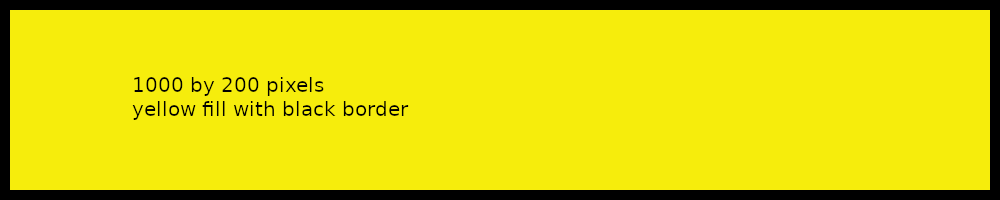
\includegraphics{1000x200} So TexWorks added the graphic right at the end of the sentence, almost literally.  Not exactly what we want, right?\\

This time, let's use the double back slash and double return, both before and after the `includegraphics' command.\\

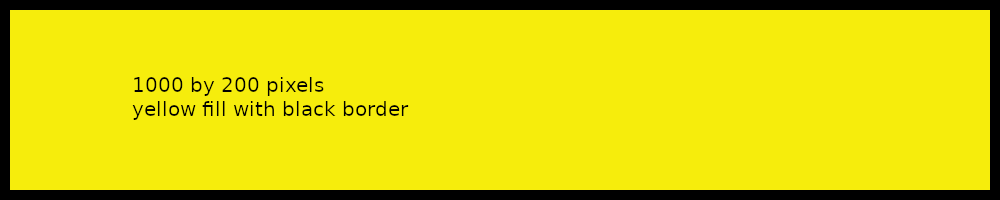
\includegraphics{1000x200}\\ % double return adds the graphic with space

That's more like it.  Why isn't our graphic centered, but instead left justified?

\section{Figures with labels and captions}

See Figure~\ref{fg:1000x200}, this figure has been entered into the .tex file after this text.  

\begin{figure}[H]
\centering
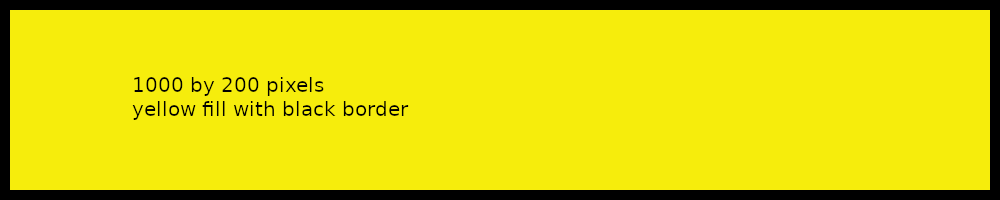
\includegraphics{1000x200}
\caption{Graphic 1000 by 200 pixels}\label{fg:1000x200}
\end{figure}

Note that the graphic is now centred on the page, even if it looks small.  Also one can see that adding a caption is easy, and referring to Figure~\ref{fg:1000x200} from within the text is also easy to do.\\

Can we do better?\\

See Figure~\ref{fg:250x250}, this figure has been entered into the .tex file after this text, and there is the extra \texttt{[H]} added to the \texttt{begin figure} command. To find out exactly what the \texttt{[H]} suffix does, delete the \texttt{[H]} that appears at the end of \texttt{begin figure}, and rebuild.  The location of the graphic will jump up above all the text on the page.

\begin{figure}[H]
\centering
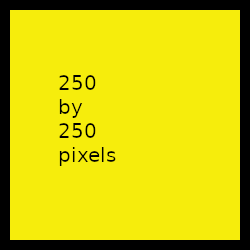
\includegraphics{250x250}
\caption{Graphic 250 by 250 pixels}\label{fg:250x250}
\end{figure}

Adding the \texttt{[H]} to the \texttt{begin figure} command tells TeXworks to turn off floating, so the figure is `anchored' by the \texttt{[H]} suffix.  The text entered after the end of the figure section then prints below the text, as you might have hoped.\\

Now if only there was a way to make that small graphic a little bigger?

\section{Scaling Figures}

See Figure~\ref{fg:250x250-2}, this figure has been scaled to one third of the width of the page.  Refer back to Figure~\ref{fg:250x250} and you can see that this graphic is much easier to read.  We scaled to the text width by entering a 0.33 scale factor to the \texttt{width =  textwidth} command. The aspect ratio has been maintained, and we didn't have to open an image editing program to change the original image size.\\

\begin{figure}[H]
\centering
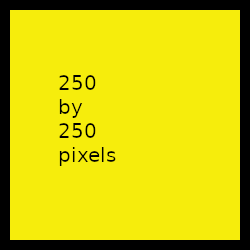
\includegraphics[width=0.33\textwidth]{250x250}
\caption{Graphic 250 by 250 pixels}\label{fg:250x250-2}
\end{figure}


If you want a full width figure, see Figure~\ref{fg:1000x200-2}, and compare the size to Figure~\ref{fg:1000x200}.

\begin{figure}[H]
\centering
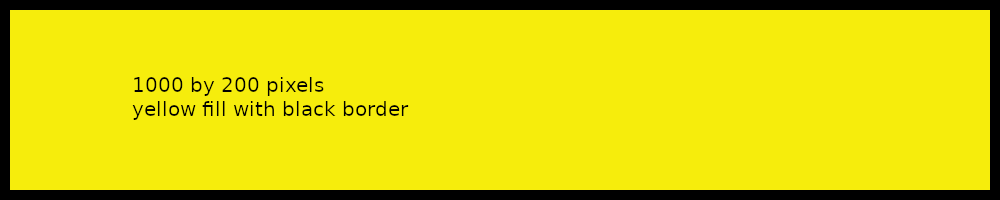
\includegraphics[width=\textwidth]{1000x200}
\caption{Graphic 1000 by 200 pixels, scaled to text width}\label{fg:1000x200-2}
\end{figure}

The graphic has been scaled up in size, so the width of the graphic matches the width of the text, using the \texttt{width = textwidth} command.  Since it is only scaling the width, the aspect ratio is maintained and now the height is greater than displayed in Figure~\ref{fg:1000x200}.\\

One can also set the width to a certain dimension, such as 150 mm, but using the text width may be a simpler way to accomplish scaling.  What if we change the document orientation from portrait to landscape, or change the paper size from A4 to Letter?  In any case, scaling can be done easily, so which method to use is up to you, the author.\\

What if you want to add two related graphics, such as two graphics that show before and after, and you want them to show up together as a single figure with a single caption?

\section{Two Figures}

\begin{figure}[H]
\centering
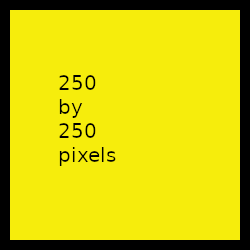
\includegraphics[width=0.35\textwidth]{250x250}
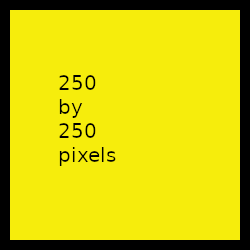
\includegraphics[width=0.35\textwidth]{250x250}
\caption{Graphic 250 by 250 pixels}\label{fg:250x250-3}
\end{figure}

\section{Three Figures}

\begin{figure}[H]
\centering
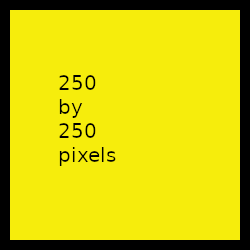
\includegraphics[width=0.3\textwidth]{250x250}
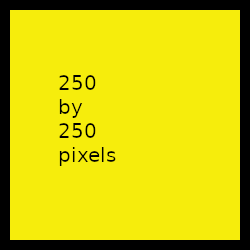
\includegraphics[width=0.3\textwidth]{250x250}
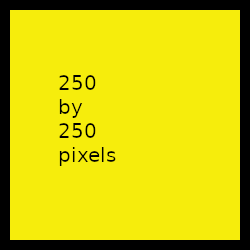
\includegraphics[width=0.3\textwidth]{250x250}
\caption{Graphic 250 by 250 pixels}\label{fg:250x250-4}
\end{figure}

\section{Four Figures}

\begin{figure}[H]
\centering
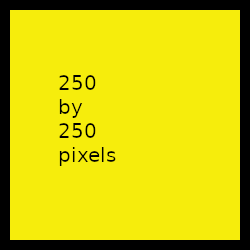
\includegraphics[width=0.2\textwidth]{250x250}
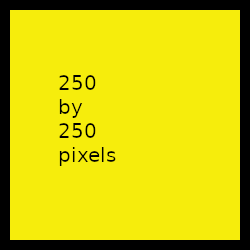
\includegraphics[width=0.2\textwidth]{250x250}
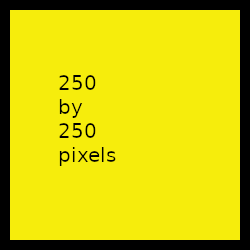
\includegraphics[width=0.2\textwidth]{250x250}
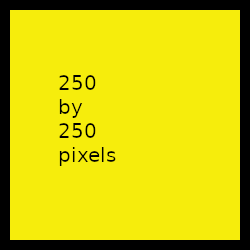
\includegraphics[width=0.2\textwidth]{250x250}
\caption{Graphic 250 by 250 pixels}\label{fg:250x250-5}
\end{figure}

Well, that was pretty easy, right?  Just adjust the width command so the total adds up to less than one, and you are in control.\\

What if you liked the size of the Two Figures, but you have four graphics that you want to display together in one figure?

% end that section and start again on a new page
\newpage

\section{Two Figures by Two Figures}

\begin{figure}[H]
\centering
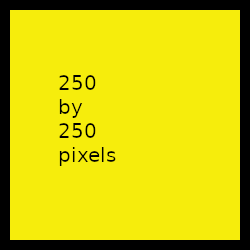
\includegraphics[width=0.33\textwidth]{250x250}
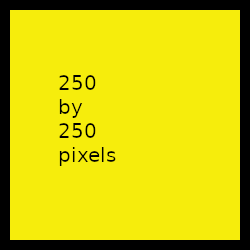
\includegraphics[width=0.33\textwidth]{250x250}
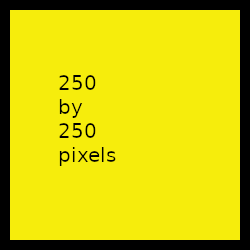
\includegraphics[width=0.33\textwidth]{250x250}
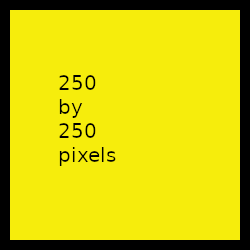
\includegraphics[width=0.33\textwidth]{250x250}
\caption{Graphic 250 by 250 pixels}\label{fg:250x250-5}
\end{figure}

That was easy.  Just increase the scale factor to 0.33 and TexWorks takes care of locating the images.  For fun, try changing the scale factor to 0.32 for all four graphics, you'll see that you get a `T' shape arrangement.\\

Next let's try stacking some graphics vertically, from top to bottom.
\begin{figure}[H]
\centering
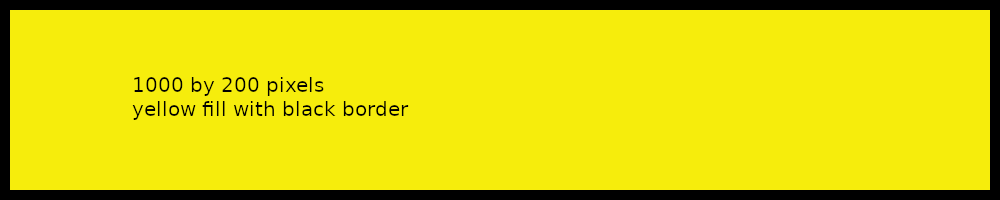
\includegraphics[width=0.9\textwidth]{1000x200}
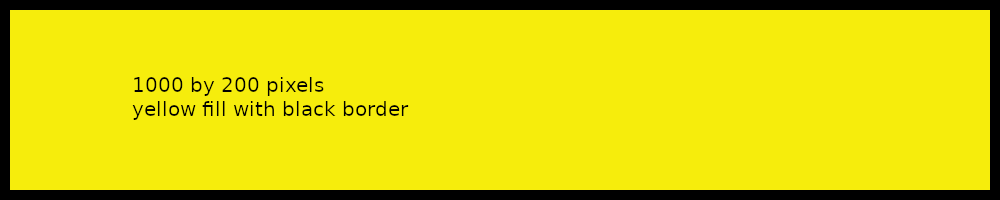
\includegraphics[width=0.9\textwidth]{1000x200}
\caption{Graphic 1000 by 200 pixels}\label{fg:1000x200-5}
\end{figure}

As you can see, it's easy to accomplish some impressive arrangements of graphics using TexWorks.\\

How about wrapping the text around the figures?

\section{Wrap Figures}

Nam dui ligula, fringilla a, euismod sodales, sollicitudin vel, wisi. Morbi auctor lorem non justo. Nam lacus libero, pretium at, lobortis vitae, ultricies et, tellus.   Nulla ullamcorper vestibulum turpis.

\begin{wrapfigure}{r}{0.4\textwidth}
\centering
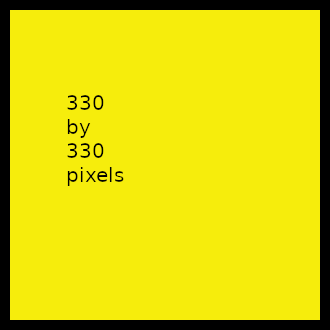
\includegraphics[width=0.3\textwidth]{330x330}
\caption{Graphic 330 by 330 pixels}\label{fg:330x330}
\end{wrapfigure}

Donec aliquet, tortor sed accumsan bibendum, erat ligula aliquet magna, vitae ornare odio metus a mi. Morbi ac orci et nisl hendrerit mollis. Suspendisse ut massa. Cras nec ante. Pellentesque a nulla. Cum sociis natoque penatibus et magnis dis parturient montes, nascetur ridiculus mus. Aliquam tincidunt urna. Pellentesque cursus luctus mauris.

Nulla malesuada porttitor diam. Donec felis erat, congue non, volutpat at, tincidunt tristique, libero. Vivamus viverra fermentum felis. Donec nonummy pellentesque ante. Phasellus adipiscing semper elit. Proin fermentum massa ac quam. Sed diam turpis, molestie vitae, placerat a, molestie nec, leo. Maecenas lacinia. Nam ipsum ligula, eleifend at, accumsan nec, suscipit a, ipsum. Morbi blandit ligula feugiat magna. Nunc eleifend consequat lorem. Sed lacinia nulla vitae enim. Pellentesque tincidunt purus vel magna. Integer non enim. Praesent euismod nunc eu purus. Donec bibendum quam in tellus. Nullam cursus pulvinar lectus. Donec et mi. Nam vulputate metus eu enim. Vestibulum pellentesque felis eu massa.\\

Once again, that wasn't too hard.  Instead of starting with \texttt{figure} we start with \texttt{wrapfigure}.  The same two parameters are needed with \texttt{wrapfigure}, just like with \texttt{wraptable}.\\

What about tables, are they easy too?

% end that section and start again on a new page
\newpage

\chapter{Tables}

\section{Tables}

Here's a table from the Rayleigh-Benard tutorial, showing the properties of water.\\

\begin{table}[h]
\caption{Material parameters for water}
\label{tb:matpar}
\centering
\begin{tabular}{ll} \hline
parameter  & value \\ \hline
density & 998.3 kg/m$^{3}$ \\
viscosity & 1040e-6 Ns/m$^{2}$ \\
heat capacity & 4183 J/(kg$\cdot$K) \\
heat conductivity & 0.58 W/(m$\cdot$K)       \\
heat expansion coefficient & 2.07e-4 K$^{-1}$      \\ 
reference temperature & 293 K       \\ \hline
\end{tabular}
\end{table}

The table is nicely centred on the page and the text entered before the table shows up before the table, and likewise the text entered  after the table shows up after the table.

\section{Wrap Tables}

There's a lot of white space to the left of the table and to the right of the table, why can't we wrap the text tightly around the table,  like you see in books and technical articles?\\

Lorem ipsum dolor sit amet, consectetuer adipiscing elit. Ut purus elit, vestibulum ut, placerat ac, adipiscing vitae, felis. Curabitur dictum gravida mauris.  Cras viverra metus rhoncus sem.

\begin{wraptable}{r}{0.45\textwidth}
\caption{Material parameters for water}
\label{tb:matpar}
\centering
\begin{tabular}{ll} \hline
parameter  & value \\ \hline
density & 998.3 kg/m$^{3}$ \\
viscosity & 1040e-6 Ns/m$^{2}$ \\
heat capacity & 4183 J/(kg$\cdot$K) \\
heat conductivity & 0.58 W/(m$\cdot$K)       \\
heat expansion coefficient & 2.07e-4 K$^{-1}$      \\ 
reference temperature & 293 K       \\ \hline
\end{tabular}
\end{wraptable}

Nam arcu libero, nonummy eget, consectetuer id, vulputate a, magna. Donec vehicula augue eu neque. Pellentesque habitant morbi tristique senectus et netus et malesuada fames ac turpis egestas. Mauris ut leo.  Nulla et lectus vestibulum urna fringilla ultrices.

Phasellus eu tellus sit amet tortor gravida placerat. Integer sapien est, iaculis in, pretium quis, viverra ac, nunc. Praesent eget sem vel leo ultrices bibendum. Aenean faucibus.  Morbi dolor nulla, malesuada eu, pulvinar at, mollis ac, nulla. Curabitur auctor semper nulla. Donec varius orci eget risus. Duis nibh mi, congue eu, accumsan eleifend, sagittis quis, diam. Duis eget orci sit amet orci dignissim rutrum.   Cras viverra metus rhoncus sem.\\

There, that wasn't too bad.  Instead of using \texttt{begin table}, we just started with \texttt{begin wraptable}.  The two entries after the \texttt{begin...} statement mean `r' for right justified, (`l' would mean left justified) and 0.45 text width means we want the table to be that wide on the page.  

For fun, experiment with `r' versus `l', and vary the width factor.  Also experiment with adding and removing  the double returns and double back slashes located at the end of the paragraph before the table block.\\

What about equations?

\chapter{Equations}

\section{Equations}

Here are some equation examples taken from some of the tutorials.\\

\noindent If you want to write the equation in line, right in a sentence in text, add the equation like this:\\

``The velocity profile at the inlet is parabolic with a mean velocity $<v_x>=1.0$~m/s and $v_y=0.0$~m/s.''\\

\noindent To place the equations with text above and text below the equations, just add the equations in between lines of text, like this:\\

``in the incompressible Navier-Stokes equation can be redefined by the Boussinesq approximation
\begin{displaymath}
\rho = {\rho}_0(1-\beta(T-{T}_0))
\end{displaymath}
where $\beta$ is the heat expansion coefficient and the subscript 0 refers to a reference state.''\\

\noindent Here's another example of equations in between lines of text, this time using the `array' command:\\

``Mathematically the problem is described by the Poisson equation
\begin{equation}
\left \{
\begin{array}{ccccc}
- \kappa \Delta T &= &\rho f & \mathrm{ in } \, \, & \Omega \\
T&=&0 & \mathrm{ on } & \Gamma
\end{array}
\right .
\end{equation}
where $\kappa$ is the heat conductivity, $T$  is the temperature and $f$ is the heat source. It is assumed that density and heat conductivity are constants.''\\

\noindent Here are two more examples of equations in between lines of text, this time with more symbols, such as the integral:\\

``This case presents solving the Laplace equation for electric potential.
\begin{equation}
  - \nabla \cdot \varepsilon \nabla \phi = 0  \, \, \, \, \in \, \, \Omega
\end{equation}
where the electric potential $\phi$ is given at conducting surfaces.  From the solution one may calculate derived fields, and capacitance which is obtained from the total electric energy 
\begin{equation}
  E=\frac{1}{2} \int \varepsilon | \nabla \phi |^2 \, d\Omega
\end{equation}
and the relation $E=CU^2/2$.''\\

\noindent Here another example of equations in between lines of text, this time with more symbols, such as the partial derivative:\\

``We solve for the temperature distribution $T$ of the glacier. A heat flux of $q=0.02$~W/m$^2$ is applied at the bottom of the glacier while the surface stays at a fixed temperature of $T_0=-10$~C. The temperature distribution in the glacier may be solved from:
\begin{equation}
\left \{
\begin{array}{cccc}
- \kappa \Delta T &= & 0 & \mathrm{ in } \, \, \Omega \\
T&=&T_0 & \mathrm{ on } \, \, \Gamma_D \\
\kappa \frac{\partial T}{\partial n} &=& q & \mathrm{ on } \,\, \Gamma_N \\
\end{array}
\right .
\end{equation}
The material properties of ice are used for the heat conductivity $\kappa(T)$.  ''\\



\section{Wrap Equations}

Wrapping text around the equations requires the use of \texttt{begin wrapfigure}, using the same suffix as for \texttt{wraptable} and \texttt{wrapfigure}.  Note that the text that belongs next to the equations must appear below the equations.\\

\begin{wrapfigure}{r}{.5\textwidth}
\begin{equation}
\left \{
\begin{array}{ccccc}
- \kappa \Delta T &= &\rho f & \mathrm{ in } \, \, & \Omega \\
T&=&0 & \mathrm{ on } & \Gamma
\end{array}
\right .
\end{equation}
\end{wrapfigure}

``Mathematically the problem is described by the Poisson equation where $\kappa$ is the heat conductivity, $T$  is the temperature and $f$ is the heat source. It is assumed that density and heat conductivity are constants.''\\

\section{Writing Equations}

LaTeX is the first and may be the best tool to write mathematical equations for publications.  There are many tutorials on the Internet describing in great detail how to write equations.  This document will not try to explain all the many ways of writing equations.\\

Be sure to visit this website:\\

\url{https://www.ctan.org/}\\

And visit the starter page:\\

\url{https://www.ctan.org/starter}

\chapter{Notes}

\section{Centering}

For those of you wondering why these examples of figures and tables use the command \texttt{centering}, instead of using the pair of commands \texttt{begin center} and \texttt{end center}, here are two examples.  As you can see, not much of a difference between them.  If you look closely, you will see that the white space at the top of Figure~\ref{fg:200x200-5} is about one line high, while the white space at the top of Figure~\ref{fg:200x200-6} is two lines high.  Really just a matter of taste, IMHO, I'd rather go with \texttt{centering} and occupy one less line in the tex source.  Many of the existing tutorials use the pair of commands \texttt{begin center} and \texttt{end center}, so once again, use the command \texttt{centering} for new tutorials and only when actually editing existing tutorials for content.

\begin{wrapfigure}{r}{0.25\textwidth}
\centering
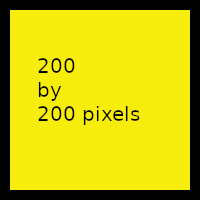
\includegraphics[width=0.25\textwidth]{200x200}
\caption{Graphic 200 by 200 pixels}\label{fg:200x200-5}
\end{wrapfigure}
Donec aliquet, tortor sed accumsan bibendum, erat ligula aliquet magna, vitae ornare odio metus a mi. Morbi ac orci et nisl hendrerit mollis. Suspendisse ut massa. Cras nec ante. Pellentesque a nulla. Cum sociis natoque penatibus et magnis dis parturient montes, nascetur ridiculus mus. Aliquam tincidunt urna. Pellentesque cursus luctus mauris.  Nulla malesuada porttitor diam. Donec felis erat, congue non, volutpat at, tincidunt tristique, libero. Vivamus viverra fermentum felis. Donec nonummy pellentesque ante. Phasellus adipiscing semper elit. Proin fermentum massa ac quam. Sed diam turpis, molestie vitae, placerat a, molestie nec, leo. Maecenas lacinia. Nam ipsum ligula, eleifend at, accumsan nec, suscipit a, ipsum. Morbi blandit ligula feugiat magna. Nunc eleifend consequat lorem. Sed lacinia nulla vitae enim. Pellentesque tincidunt purus vel magna. Integer non enim. Praesent euismod nunc eu purus. Donec bibendum quam in tellus. Nullam cursus pulvinar lectus. Donec et mi. Nam vulputate metus eu enim. Vestibulum pellentesque felis eu massa. Nam dui ligula, fringilla a, euismod sodales, sollicitudin vel, wisi. Morbi auctor lorem non justo. Nam lacus libero, pretium at, lobortis vitae, ultricies et, tellus.   Nulla ullamcorper vestibulum turpis. Nam dui ligula, fringilla a, euismod sodales, sollicitudin vel, wisi. Morbi auctor lorem non justo. Nam lacus libero, pretium at, lobortis vitae, ultricies et, tellus.
\begin{wrapfigure}{r}{0.25\textwidth}
\begin{center}
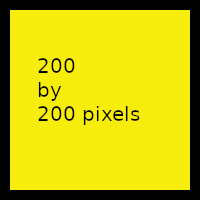
\includegraphics[width=0.25\textwidth]{200x200}
\caption{Graphic 200 by 200 pixels}\label{fg:200x200-6}
\end{center}
\end{wrapfigure}

Donec aliquet, tortor sed accumsan bibendum, erat ligula aliquet magna, vitae ornare odio metus a mi. Morbi ac orci et nisl hendrerit mollis. Suspendisse ut massa. Cras nec ante. Pellentesque a nulla. Cum sociis natoque penatibus et magnis dis parturient montes, nascetur ridiculus mus. Aliquam tincidunt urna. Pellentesque cursus luctus mauris. Nulla malesuada porttitor diam. Donec felis erat, congue non, volutpat at, tincidunt tristique, libero. Vivamus viverra fermentum felis. Donec nonummy pellentesque ante. Phasellus adipiscing semper elit. Proin fermentum massa ac quam. Sed diam turpis, molestie vitae, placerat a, molestie nec, leo. Maecenas lacinia. Nam ipsum ligula, eleifend at, accumsan nec, suscipit a, ipsum. Morbi blandit ligula feugiat magna. Nunc eleifend consequat lorem. Sed lacinia nulla vitae enim. Pellentesque tincidunt purus vel magna. Integer non enim. Praesent euismod nunc eu purus. Donec bibendum quam in tellus. Nullam cursus pulvinar lectus. Donec et mi. Nam vulputate metus eu enim. Vestibulum pellentesque felis eu massa. Nam dui ligula, fringilla a, euismod sodales, sollicitudin vel, wisi. Morbi auctor lorem non justo. Nam lacus libero, pretium at, lobortis vitae, ultricies et, tellus.   Nulla ullamcorper vestibulum turpis. Nam dui ligula, fringilla a, euismod sodales, sollicitudin vel, wisi. Morbi auctor lorem non justo. Nam lacus libero, pretium at, lobortis vitae, ultricies et, tellus.   Nulla ullamcorper vestibulum turpis.

\section{The beginning}

That's it for these instructions.  If you need something more complicated that these examples, then I'm sure you will find an answer somewhere on the Internet.  Consider adding what you have found into this document, to expand on these few examples.\\

If you search the Internet for `texworks equations', you will find lot's of references, such as:\\

\url{https://www.overleaf.com}\\

\url{https://en.wikibooks.org}\\

\url{https://tex.stackexchange.com}\\

\url{https://latex-tutorial.com}\\

\url{https://www1.cmc.edu}\\

\url{https://www.authorea.com}\\




 
 
%\phantomsection % sets an anchor
%\addcontentsline{toc}{part}{Index} % Include the index in TOC

%\printindex


\end{document}

